\section{Introduction}
% Your task is to use the bullet points blwloe to craft a paragraph that introduces my paper. This paragraph should introduce the topic of pairs trading, and review it in the context of the paper by Gatev. It should sound like a reexamination of the idea of pairs trading two decades after the publication of the seminal paper by Gatev. Note that text enclosed in \bblue{} are literally extracted from the original paper, so using them literally constitutes plagiarism: instead, either you should aim to rephrase the ideas inferred from the \bblue{} text and rephrase them / apply them in a differnt style, or you could cite them literally between quotes.

% Also, replace mentions to references by citations: 
% Gatev et al: \cite{Gatev2006}
% Do and Faff: \cite{Do2010}

\paragraph{Revisiting pairs trading 20 years after Gatev et al.}
\begin{itemize}
\item As documented in Gatev et al 
\begin{itemize}
\item \bblue{Pairs trading was developed in the mid-1980s by Nunzio Tartaglia to uncover arbitrage opportunities in the equity markets. }
\item \bblue{Since then, pairs trading became an increasingly popular \qquote{market neutral} investment strategy used by individual and institutional trades as well as hedge funds.}
\item \bblue{pairs trading was a poopular short-term speculation strategy with long years of history in Wall Street, belonging to the propietary \qquote{statistical arbitrage} tools used by hedge funds and investment banks}
\end{itemize}

\item \bblue{The concept of pairs trading is disarmingly simple. Find two stocks whose prices have moved together historically. When the spread between them widens, short the winner and buy the loser. If history repeats itself, prices will converge and the arbitrageur will profit}. In other words, if Stock $A$ and $B$ historically trade at a 1:1 ratio but temporarily diverge to 1:1.05, arbitrageurs short the overvalued stock and buy the undervalued one. The tiny profit margin (e.g., 0.05\% gain) justifies the trade, restoring the 1:1 ratio.

\item \bblue{It is hard to believe that such a simple strategy, based solely on past price dynamics and simple contrarian principles, could possibly make money. If the U.S. equity market were efficient at all times, risk-adjusted returns from pairs trading should not be positive.} Yet Gatev et al find average annualized excess returns of about 11\% for top pairs portfolios. 

\item Gatev already documented that \bblue{the increased popularity of quantitative-based statistical arbitrage strategies has also apparently affected profits.}

\begin{itemize}
\item 20 years after the publication of Gatev's paper, we can substantiate this: ever since the publication of the seminal paper by Gatev et al. and a later reexamination by Do and Faff, this practice has been completely arbitraged away, and pairs trading is no longer profitable. Finding those pairs has become increasingly difficult in the past decade. The Figure below shows the evolution of monthly excess returns to pairs trading from 1962 to 2025, evidencing that, in the last decade, pairs trading is no longer profitable.
\item This is similar to what happened with the momentum strategy: ever since the seminal paper was published, the strategy got popularized, and markets became much more efficient.
\end{itemize}

%(as we see in the graph, making money in pairs trading has become more and more difficult in the past years, perhaps because the market for pairs trading has become too known and hadge funds have depleted the arbitrage opportunities, or perhaps is a new tendency of stocks to become more unique (and less directly substitutable) in the last decade
\end{itemize}

\begin{figure}[H]
\centering
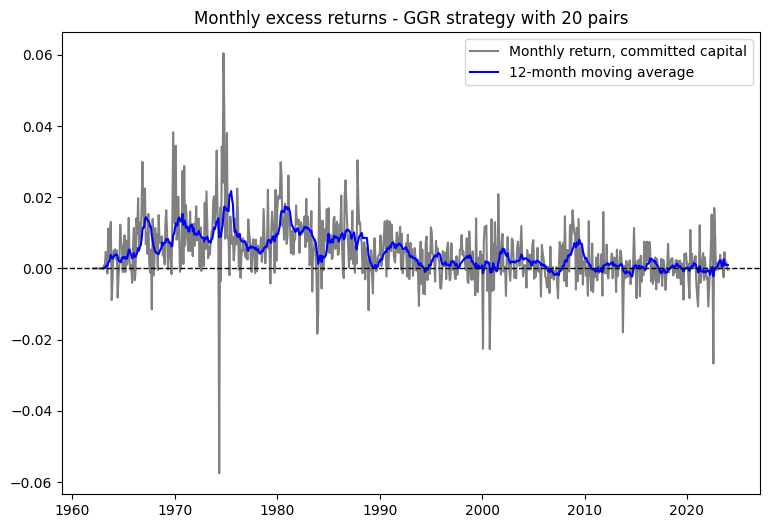
\includegraphics[scale=0.8]{fig_pairs_trading_evolution.png}
\end{figure}



\paragraph{Generalizing Pairs Trading}
However, the essence of the idea--trading the spread between two assets that are related-- can be generalized. We could take a stock, say, General Motors, and instead of looking for another stock whose \textit{normalized} price series behaves similarly to that of General Motors, we could simply try to reconstruct the \textit{normalized} price series of General Motors as a linear combination of those of other stocks. That is, a simple linear regression where we regress the price of General Motors onto the prices of a selection of assets would allow us to closely replicate the price of the first. 

Similar to traditional pairs trading, this idea is also rooted in asst pricing theory. In particular, in the framework of relative pricing, where we consider that two securities are close substitutes to each other. In the case of pairs trading, we try to find one stock which could deem as "substitute" of the target stock, whereas my idea is more flexible, ins the sense that it allows to construct a synthetic substitute from a linear combination of other stocks. In either case, the mission of finding a substitute can be relaxed by not imposing such a severe cardinality constrain! Note that in the case of pairs trading, we impose a severe cardinality constraint where we limit the reconstruction of the substitue of a target asset to a unique other asset. However, if we relax this constraint and allow ourselved to find such a substitute using more assets, we can create a synthetic replica of the original stock, such that the spread between the original asset and its replica satisfies some nice and desirable properties for profitable trading. In particular, we know that the residual in an OLS regression has 0 mean by construction in the formation sample, if we exploit the estimates of the OLS regression out of sample for a reduced time period, we can hope that those residuals maintain those nice properties, and hence, we could trade the regression residual by betting on it mean reversion to 0.


Hence, this paper proposes a novel framework rooted in asset pricing theory to pairs trade a target asset against a synthetic replica built as a linear combination of other stocks. Because trading a large pool of assets is costly, we obviously want to limit the cardinality of the donor pool of assets that constitute the replica. Pairs trading is the extreme case, where such cardinality constraint is set equal to 1. We propose a more flexible framework where we impose a lasso penalty on the OLS regression to promote sparsity in our solution, without restricting the solution with hard cardinality constraints. Lasso has some nice properties and is ideal in this context, where we aim to select the stocks that contribute the most to the replication of the target asset without the curse of dimensionality of using too many assets, which would turn our trading strategy unfeasible. 


\paragraph{Data snooping and market response}
Our methodology replicates the core application from Gatev et al, and adapts it to the case where the cardinality constraint in the lookup for a substitute of the target asset is relaxed.
As in Gatev, we also have abstracted away from searching over the full strategy space to identify successful trading rules. Instead, we have adapted the same parameterization and rules proposed by Gatev. In their paper, Gatev et al argue that their rules follow the feneral outline:

\begin{itemize}
\item First. \qquote{\bblue{Find stocks that move together}}. In traditional pairs trading this is done by finding two ``real'' pairs. In our case, this is done by constructing a synthetic replica of a target asset.
\item Second. \qquote{\bblue{Take a long-short position when they diverge and unwind on convergence}}. In our case, this is equivalent to betting on the mean reversion of the regression residual. That is, we go short when the regression error is positive, and long otherwise.
\end{itemize}



Similar to Gatev et al, we account for transaction costs indirectly by waiting one day after the signal from the pairs trade is derived. 	


\paragraph{Relative pricing}
% Rooting the idea in Asset Pricing theory
Asset pricing can be viewed in absolute and relative terms. 

\begin{itemize}
\item \bblue{Absolute pricing values securities from fundamentals such as discounted future cash flow. This is a notoriously diffucult process with a wide margin for error.}
\item \bblue{Relative pricing is only slightly easier. Relative pricing means that two securities that are close substitutes for each other should sell for the same price --it does not say what that price will be. Thus, relative pricing allows for bubbles in the economy, but not necessarily arbitrage or profitable speculation. The Law of One Price [LOP] and a ``near-LOP'' are applicable to relative pricing, even if that price is wrong.}
\begin{itemize}
\item \bblue{Ingersoll (1987) defines the LOP as the ``proposition ... that two investments with the same payoff in every state of nature must have the same current value.'' In other words, two securities with the same prices in all states of the world should sell for the same amount.}
\item \bblue{Chen and Knez (1995) extend this to argue that ``closely integrated markets should assign to similar payoffs prices that are close''. They argue that two securities with similar, but not necessarily, matching payoffs across states should have similar prices. This is of course a weaker condition and subject to bounds on prices for unusual states; however, it allows the examination of ``near-efficient'' economies, or in Chen and Knez' case, near integrated
markets. Notice that this theory corresponds to the desire to find two
stocks whose prices move together as long as we can define states of
nature as the time series of observed historical trading days.} In traditional pairs trading, we need to find two stocks with near-matching payoffs, which is of a complicated nature due to the fact that we are restricted to exclusively one. On the other hand, finding a matching payoff from a combination of assets is much easier. In a near efficient economy (i.e.: if markets are integrated), the price of the target asset should match that of its synthetic replica.
\end{itemize}
\end{itemize}


\paragraph{Co-integrated prices}

As mentioned in Gatev et al, \bblue{the pairs trading strategy may be justified within an equilibrium asset-pricing framework with nonstationary common factors like Bossaerts and Green (1989) and Jagannathan and Viswanathan (1988).}

% WORK IN UNDERSTANDING THIS
\bblue{If the long and short components fluctuate with common nonstationary factors, then the prices of the component portfolios would be co-integrated and the pairs trading strategy would be expected to work. Evidence of exposures to common nonstationary factors would support a nonstationary factor pricing framework.

The space of normalized, cum-dividend prices, that is, cumulative total returns with dividends reinvested, is the basic space for the pairs trading strategies in this article. The main observation about our motivating models of the CAPM-APT variety is that they are known to imply perfect collinearity of prices, which is readily rejected by the data. On the other hand, Bossaerts (1988) finds evidence of price co-integration for the U.S. stock market. We would like to keep the notion of the empirically observed co-movement of prices, without unnecessarily restrictive assumptions, hence we proceed in the spirit of the co-integrated prices literature.


More specifically, our matching in price space can be interpreted as follows. Suppose that prices obey a statistical model of the form
$p_{i t}=\sum \beta_{i l} p_{l t}+\varepsilon_{i t}, k<n$
where $\varepsilon_{i t}$ denotes a weakly dependent error in the sense of Bossaerts (1988). Assume also that $p_{i t}$ is weakly dependent after differencing once. Under these assumptions, the price vector $\boldsymbol{p}_{\boldsymbol{t}}$ is co-integrated of order 1 with cointegrating rank $r=n-k$, in the sense of Engle and Granger (1987) and Bossaerts (1988). Thus, there exist $r$ linearly independent vectors $\left\{\boldsymbol{\alpha}_q\right\}_{q=1, \ldots, r}$ such that $z_q=\boldsymbol{\alpha}_q{ }^{\prime} \boldsymbol{p}_t$ are weakly dependent. In other words, $r$ linear combinations of prices will not be driven by the $k$ common nonstationary components $p_l$. Note that this interpretation does not imply that the market is inefficient, rather it says that certain assets are weakly redundant, so that any deviation of their price from a linear combination of the prices of other assets is expected to be temporary and reverting.

To interpret the pairs as co-integrated prices, we need to assume that for $n \gg k$, there are co-integrating vectors that have only two nonzero coordinates. In that case, the sum or difference of scaled prices will be reverting to zero and a trading rule could be constructed to exploit the expected temporary deviations. Our strategy relies on exactly this conclusion. In principle one could construct trading strategies with trios, quadruples, and so on of stocks, which would presumably capture more co-integrated prices and would yield better profits.
}

\subsection{Cointegration Meets Synthetic Controls: A Formal Equivalence}
\label{sec:cointegration_meets_synthetic_controls}

In this appendix section, we develop a formal argument showing how, under some stringent assumptions, our notion of \emph{synthetic control} can be viewed as a special case of \emph{cointegration}. This connection underlies the intuition that, when one normalizes the first variable of a cointegrated system to 1, the remaining cointegration relationships effectively produce the \emph{synthetic} version of the first variable when the cointegration vector satisfies a specific restriction. 
%Here, we adopt a rigorous perspective aimed at bridging the econometric concept of cointegration with methodologies employed in the synthetic control literature (e.g., Abadie and Gardeazabal).

%\subsection{Cointegration}

Let $\{y_{i,t} \}_{t=1}^{T}$ denote the time series sequence of log-prices for each asset $i\in\{1,\ldots,N\}$.
%
Throughout, we assume each $y_{i,t}$ is an $I(1)$ process (integrated of order 1). 
%
Formally, an $I(1)$ process is one that becomes \emph{stationary} (and typically ergodic) upon differencing once:
$\Delta y_{i,t} := y_{i,t} - y_{i,t-1} \sim I(0).$
%
The notion of cointegration, due to Engle and Granger, is central in analyzing potentially long-run equilibria among these variables.

%----------------------------------------------------
\begin{definition}[Engle and Granger (1987)]
The components of $\mbf{y}_t:=[y_{1t}, ..., y_{Nt}]$ are said to be cointegrated of order $d$, $b$, denoted $\mbf{y}_t \sim CI(d,b)$, if (a) all components of $\mbf{y}_t$ are $I(d)$ and (b) a vector $\b{\beta}\neq 0$ exists so that $\b{\beta}'\mbf{y}_t \sim I(d-b)$, $b > 0$. The vector $\b{\beta}$ is called the cointegrating vector.
\end{definition}
%----------------------------------------------------
%\begin{definition}[Campbell and Perron (1991)]
%An $(n \times 1)$ vector of variables $\mbf{y}_t$ is said to be cointegrated if at least one nonzero $n$-element vector $\b{\beta}_i$ exists such that $\b{\beta}'_i\mbf{y}_t$ is trend-stationary. $\b{\beta}_i$ is called a cointegrating vector. If $r$ such linearly independent vectors $\b{\beta}_i(i = 1,\ldots,r)$ exist, we say that $\{\mbf{y}_t\}$ is cointegrated with cointegrating rank $r$. We then define the $(n \times r)$ matrix of cointegrating vectors $\b{\beta} = (\b{\beta}_1,\ldots,\b{\beta}_r)$. The $r$ elements of the vector $\b{\beta}'\mbf{y}_t$ are trend-stationary, and $\b{\beta}$ is called the cointegrating matrix.
%\end{definition}
%----------------------------------------------------

%\subsection{Synthetic Control}
%\begin{definition}
%In a synthetic control problem we have a target element $y_1$ that we seek to mimick through a linear combination of elements in a donor pool $\mbf y_{2:n}=(y_2,...,y_n)$ with weigths $\mbf w=\arg\underset{w\in\W}{\min} \sum_{t=1}^T (y_1-\mbf w'\mbf y_{2:n})^2$ where $\mathcal{W} := \{\mbf{w}\in\mathbb{R}_{+}^{n-1}: \sum_{j=2}^n w_j=1\}$.
%\end{definition}

\begin{definition}[Synthetic Control]\label{def:synthetic_control}
Let $\{y_1, y_2, \dots, y_n\}$ be a collection of random variables, where $y_1$ is the ``target'' variable and 
$\mathbf{y}_{2:n} = (y_2,\dots,y_n)$ constitute the ``donor pool''. A \emph{synthetic control} for
$y_1$ is constructed by choosing weights $\mathbf{w}$ in the $(n-1)$-dimensional space
$\mathcal{W} := \{\mbf{w}\in\mathbb{R}_{+}^{n-1}: \sum_{j=2}^n w_j=1\}$
that satisfy
%to minimize the sum of squared deviations over $T$ observations:
$\mbf w=\arg\underset{w\in\W}{\min} 
\sum_{t=1}^T 
(y_{1,t}-\mbf w'\mbf y_{2:n,t})^2$.
%Because $\mathcal{W}$ is precisely the convex hull of the standard basis vectors in $\mathbb{R}^{n-1}$, the resulting synthetic control $\mathbf{w}'\,\mathbf{y}_{2:n}$ is a convex combination of the donor pool elements $(y_2,\dots,y_n)$.
\end{definition}


%\subsection{Equivalence}
Given that cointegration relationships prevail up to scale and sign changes, then, under suitable conditions on the cointegration vector, there exists a nontrivial constant $\kappa$ that allows us to reinterpret the cointegration relationship as one of a synthetic control. In particular,
%----------------------------------------------------
\begin{proposition} 
For a cointegrated vector $\mbf y$  with rank $r$, if (at least) one of the cointegrating vectors $\b \beta$ satisfies the restriction
$\mathcal R=
\{
%\begin{array}{ll}
%\b \beta > 0, ~
\mbf 1' \b \beta  = 0
%\\
%\beta_j \geq 0, j\neq i
%\end{array}
\}$,
%( i.e, that its components 
%are nonnegative and 
%sum to 1
%, and at least one of them is strictly positive). 
 then we can scale the cointegration vector by $\kappa=1/\beta_i$ such that $\kappa \b \beta ' \mbf y$ is stationary and describes a \qquote{synthetic control} relationship (as per \cref{def:synthetic_control}) between $y_i$ and $\mbf y_{-i}$. 
\end{proposition}
%----------------------------------------------------

\begin{proof}
The proof is straightforward. For a cointegration vector $\b \beta$ where $\mathcal R$ holds, we have that $\mbf 1'\b \beta = \sum_{j=1}^n \beta_j= 0$, which trivially implies $\beta_i = -\sum_{j\neq i}\beta _j$. For the sake of the proof, set that $\beta_i$ to the first component ($\beta_1$). Then
$\beta_1 = -\sum_{j=2}^n \beta_j$ and $\kappa = (\beta_1)^{-1} = -(\sum_{j=2}^n \beta_j)^{-1}$
$$
\kappa \b \beta' \mbf y 
= 
\frac{1}{\beta_1} [\beta_1 ~~ \b \beta_{2:n}] \mbf y_t 
=
\2{1 ~~ \frac{-\b \beta'_{2:n}}{\sum_{j=2}^n\beta_j}}
\2{\v{y_1 \\ \mbf y_{2:n}}}
=
y_1 - \frac{\beta_2}{\sum_{j=2}^n \beta_j}y_2 - \cdots - 
\frac{\beta_n}{\sum_{j=2}^n \beta_j} y_n
\sim I(0)
$$
describes a stationary cointegration relationship in $\mbf y$, and since
\begin{align*}
y_1 
&= \frac{\beta_2}{\sum_{j=2}^n \beta_j}y_2 + \cdots + 
\frac{\beta_n}{\sum_{j=2}^n \beta_j} y_n + \eps 
\\&= \mbf w' \mbf y_{2:n} + \eps 
%, \t{~~where~} \eps\sim I(0)
\end{align*}
with $\eps\sim I(0)$ and $\mbf w:=\1{\frac{\beta_2}{\sum_{j=2}^n \beta_j}, ..., \frac{\beta_n}{\sum_{j=2}^n \beta_j}}'\in \W$, then this relationship is endowed with a synthetic control structure. A similar reasoning applies to any other $\beta_i$ different from $\beta_1$.
\end{proof}


This paper constitutes an extension of pairs trading and an empirical investigation of this last statement in Gatev et al. If prices are really cointegrated, as found in Bossaerts (1988), then, any deviation of the prices from this cointegration relationship should allow us to trade profitably by betting against that deviation.

